\documentclass[tikz,margin=1mm]{standalone}
\usetikzlibrary{matrix}
\tikzset{
    every matrix/.style={
        inner sep=-\pgflinewidth,
        matrix of math nodes,
        column sep=-\pgflinewidth,
        nodes={
            draw=black,
            font=\color{black},
            minimum size=.8cm,
            minimum width=1.4cm,
            anchor=center
        }
    }
}
\begin{document}
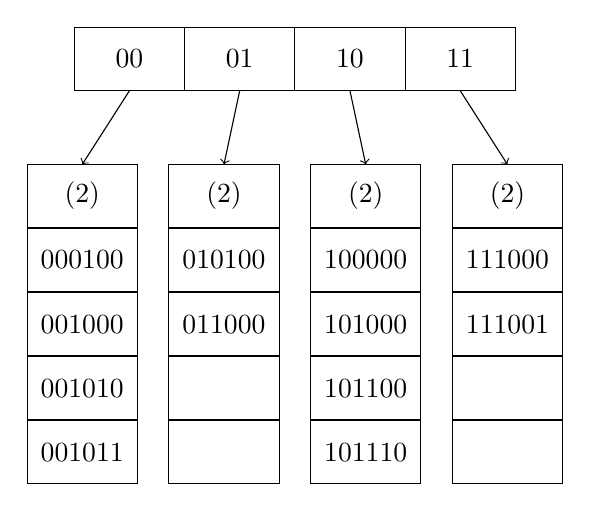
\begin{tikzpicture}
\matrix[above] (t1) at (0,0) {00 & 01 & 10 & 11\\};

\matrix[above] (t21) at (-2.7,-5) {(2) \\ 000100 \\ 001000 \\ 001010 \\ 001011 \\};
\matrix[above] (t22) at (-0.9,-5) {(2) \\ 010100 \\ 011000 \\ \  \\ \  \\};
\matrix[above] (t23) at (0.9,-5) {(2) \\ 100000 \\ 101000 \\ 101100 \\ 101110 \\};
\matrix[above] (t24) at (2.7,-5) {(2) \\ 111000 \\ 111001 \\ \  \\ \  \\};

\draw[->,black](t1-1-1.south) -- (t21.north);
\draw[->,black](t1-1-2.south) -- (t22.north);
\draw[->,black](t1-1-3.south) -- (t23.north);
\draw[->,black](t1-1-4.south) -- (t24.north);
\end{tikzpicture}
\end{document}